% The decomposition group D_𝔭 inside G = Gal(K/ℚ), isomorphic via θ
% to the cyclic group ⟨T | T^f = 1⟩, sending Frob_𝔭 to T.
% Source: book/tex/alg-NT/frobenius.tex (§ Frobenius elements) — asy.
\documentclass[border=2mm]{standalone}
\usepackage{tikz}
\usetikzlibrary{arrows.meta}
\usepackage{amssymb}
\usepackage{amsmath}
\begin{document}
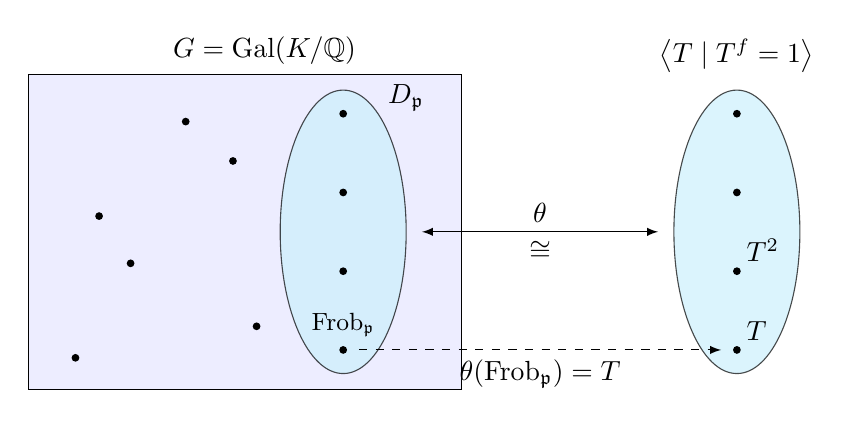
\begin{tikzpicture}[>=latex]
  % Big box for G.
  \filldraw[fill=blue!7, draw=black] (-4,-2) rectangle (1.5,2);
  \node[anchor=south] at (-1,2) {$G = \operatorname{Gal}(K/\mathbb{Q})$};
  \fill (-1.1,-1.2) circle (1.4pt);
  \fill (-1.4,0.9) circle (1.4pt);
  \fill (-2,1.4) circle (1.4pt);
  \fill (-2.7,-0.4) circle (1.4pt);
  \fill (-3.1,0.2) circle (1.4pt);
  \fill (-3.4,-1.6) circle (1.4pt);
  % D_p ellipse.
  \filldraw[fill=cyan!20, draw=black, opacity=0.7] (0,0) ellipse (0.8 and 1.8);
  \node[anchor=north] at (0.8,2) {$D_{\mathfrak{p}}$};
  \foreach \y in {-1.5,-0.5,0.5,1.5} { \fill (0,\y) circle (1.4pt); }
  \node[anchor=south] at (0,-1.45) {\small $\operatorname{Frob}_{\mathfrak{p}}$};
  % Cyclic group ellipse.
  \filldraw[fill=cyan!20, draw=black, opacity=0.7] (5,0) ellipse (0.8 and 1.8);
  \node[anchor=south] at (5,1.9) {$\left\langle T \mid T^f = 1 \right\rangle$};
  \foreach \y in {0.5,1.5} { \fill (5,\y) circle (1.4pt); }
  \fill (5,-1.5) circle (1.4pt) node[anchor=south west] {$T$};
  \fill (5,-0.5) circle (1.4pt) node[anchor=south west] {$T^2$};
  % Isomorphism arrows.
  \draw[<->] (1,0) -- (4,0);
  \node[anchor=south] at (2.5,0) {$\theta$};
  \node[anchor=north] at (2.5,0) {$\cong$};
  \draw[->, dashed] (0.2,-1.5) -- (4.8,-1.5);
  \node[anchor=north] at (2.5,-1.5) {$\theta(\operatorname{Frob}_{\mathfrak{p}}) = T$};
\end{tikzpicture}
\end{document}
